\documentclass{beamer}
\setbeamercolor{background canvas}{bg=black}
\setbeamertemplate{navigation symbols}{}
\usepackage{tikzlings}
\begin{document}
	
\begin{frame}

\begin{tikzpicture}[remember picture, overlay]

\node[opacity={0.75+0.5*sin(10*\thepage)}] at (current page.center) {
\includegraphics[width=\paperwidth]{stars}};
\node[opacity={0.75+0.5*cos(10*\thepage)}] at (current page.center) {
\includegraphics[width=\paperwidth,page=2]{stars}};

\node at (9*\thepage/100,-4+6.5*\thepage/100) {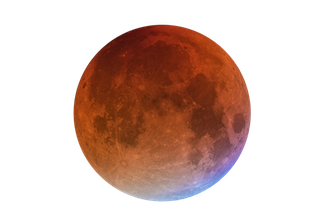
\includegraphics[width=3cm]{moon}};
\node[opacity=0.6,xshift=1cm,yshift=-0.5cm] at (9*\thepage/100,-4+6.5*\thepage/100) {
\includegraphics[width=20cm]{halo}};

\node at (current page.center) {
\includegraphics[width=\paperwidth]{montain}};

%\fill[darkgray!\thepage!black] (5,-5.5) ellipse (7 and 1.3);

\cat[body=gray!\thepage!black,yshift=-5cm,xshift=1cm,nose=red!40!white!80!gray!\thepage!black,whiskers=black]



\end{tikzpicture}

\pause[100]
	
\end{frame}	

\end{document}